\section{Streaming}

\begin{figure}[!t]
    \centering
    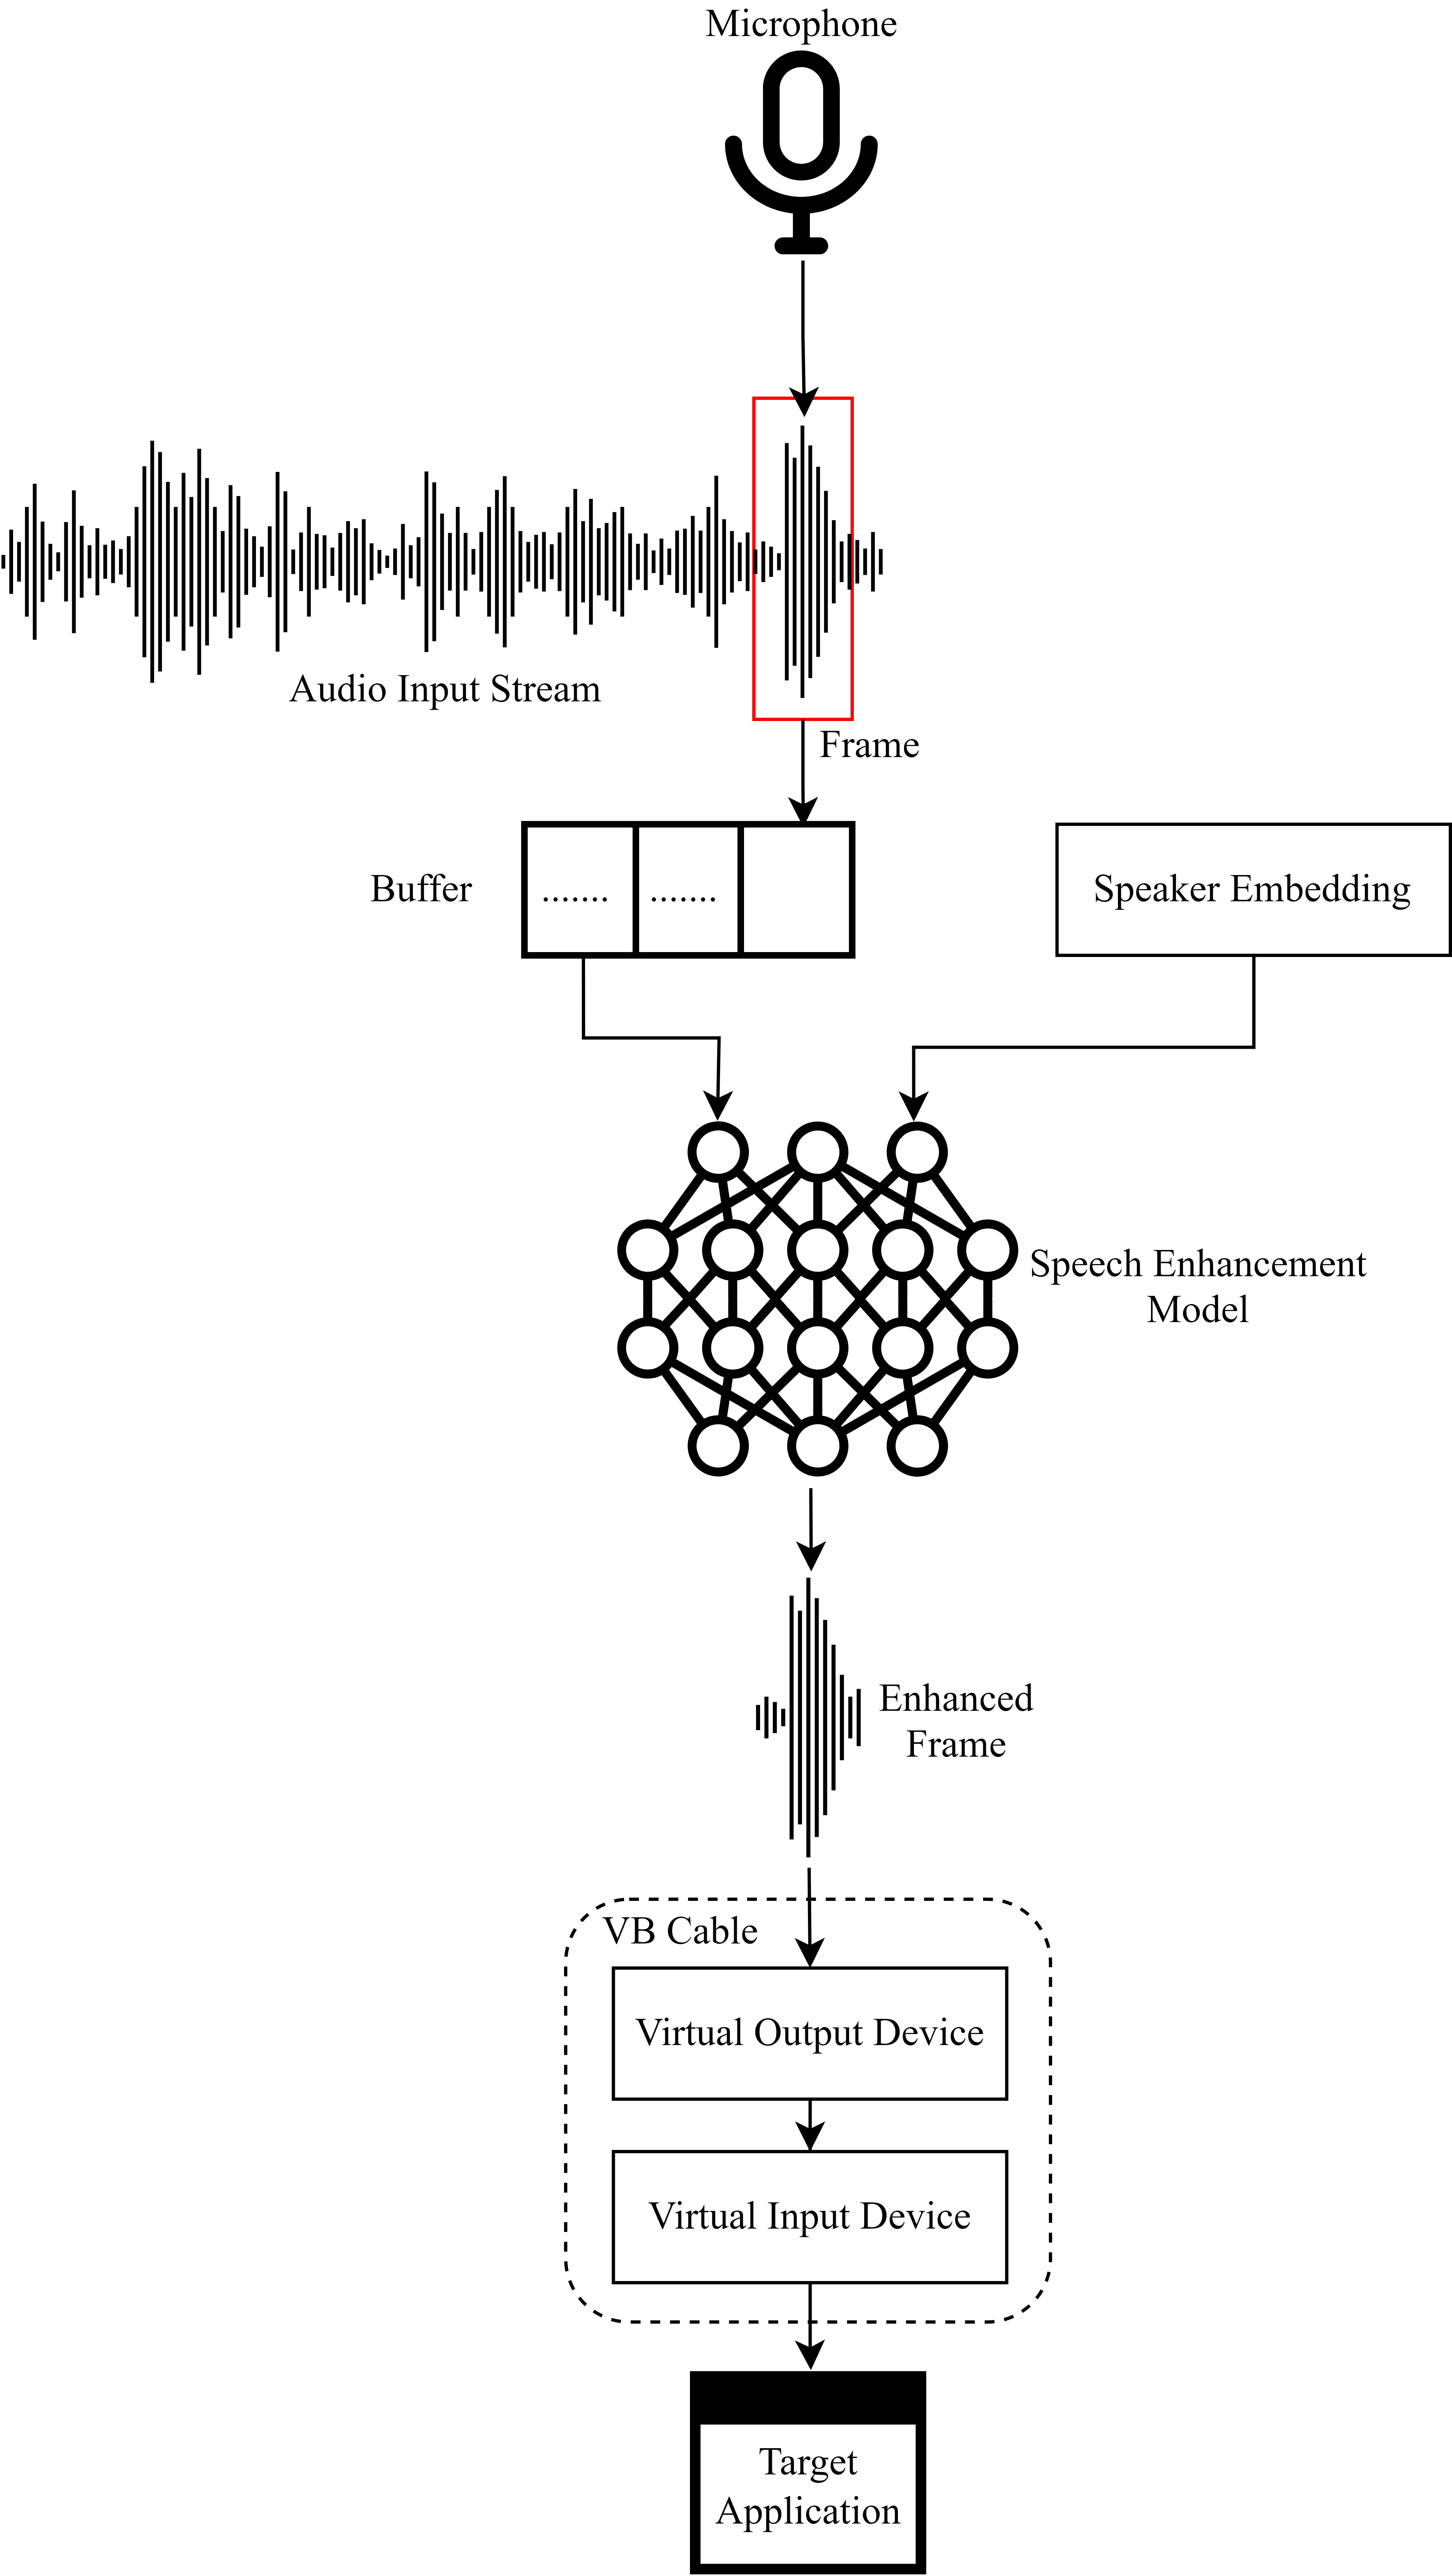
\includegraphics[width=0.8\textwidth]{images/application/streaming_pipeline.png}
    \caption{Streaming pipeline}
    \label{fig:streaming-pipeline}
\end{figure}

The streaming module is responsible for capturing real-time audio input from the user and feeding it into the machine learning model for processing. The streaming module is designed to efficiently manage and stream the audio data, ensuring that it is continuously fed into the system without interruptions. This section provides an overview of the streaming module, detailing its primary components and functionality.

The steaming pipeline starts from the user's microphone, which captures the audio input. The streaming module collects small chunks of audio data, called frames, from the microphone. Typically, the frame size is set to 60 milliseconds, however this value can be adjusted according to the application requirements. There is a trade-off between the frame size, the latency and the performance of the system. A smaller frame size will result in lower latency. Also, longer frames will result in better overall audio quality processed by the model since the model will have more context to work with but will increase the latency.

The gathered audio frames are then continuously pushed into a buffer. The buffer is a queue-like data structure that stores the audio frames in a first-in-first-out (FIFO) order. The buffer ensures that the audio frames are processed in the order they were received. Concurrent with the buffer, the streaming module continuously feeds the audio frames into the machine learning model for processing. The enhanced audio frames are then passed to the virtual output device. The virtual output device is responsible for rerouting the processed audio frames to the virtual microphone, which is then used by the user's applications as the input device. Figure \ref{fig:streaming-pipeline} shows the streaming pipeline.

In order to increase the quality of the enhanced audio, we added the option to process multiple audio frames at the same time. This increases the context the model has to work with, which results in better audio quality. As mentioned earlier, this comes at the cost of increased latency because the output device waits until $n$ full frames are gathered, making the latency as follows:
$$ \text{latency} = n \times \text{frame length} + n \times \text{processing time per frame} $$
To mitigate this, instead of keeping the streaming module idle while waiting for the model to process the audio frames, we start by processing the first frame and then save this frame for future processing. The $n-1$ saved past frames are then concatenated to the new frame to be processed by the model. This way, the streaming module can continue to collect and process audio frames without waiting for the full $n$ frames to arrive making the overall latency:
$$ \text{latency} = \text{frame length} + n \times \text{processing time} $$
This allows the streaming module to keep up with the real-time audio input and reduce the overall latency of the system. However, this approach may introduce a delay due to the added processing time of the model. This added delay is way less than the latency introduced by waiting for the full $n$ frames to arrive since the processing time is typically less than the frame length to achieve real-time constraints. We also added the option to adjust the number of working threads to process the audio frames. This far reduces the processing time of the model, which results in lower latency. If the user set the number of threads to $n$, the model will process $n$ frames at the same time, which will result in a latency of almost:
$$ \text{latency} = \text{frame length} + \text{processing time} $$
This will result in the lowest latency possible, almost the same as processing 1 frame at a time. However, it will require more processing power.

In our experiments, we set number of frames $n$ to $2$ and number of threads to $2$. This configuration resulted in a low RTF of $0.21$, which is excellent for real-time applications with low CPU utilization of $4\%$. This experiment was conducted on a laptop with CPU AMD Ryzen 9 5900HX. We can further reduce the latency and RTF by using GPU acceleration.